
\begin{multicols}{2}
Sur la figure ci-contre, qui n'est pas en
vraie grandeur:\\
$IR=8$~cm, $RP=10$~cm, $IP=4,8$~cm, $IM=4$~cm,
$IS=10$~cm, $IN=6$~cm et $IT=6$~cm.\\
\textit{(On ne demande pas de refaire la figure.)}
\begin{enumerate}
\item Démontre que les droites $(ST)$ et $(RP)$ sont parallèles.
\item Déduis-en la longueur $ST$.
\item Les droites $(MN)$ et $(ST)$ sont-elles parallèles ? Justifie.
\end{enumerate}
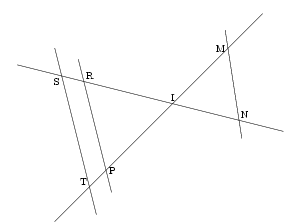
\includegraphics[scale=1]{TR-exo29.png} 
\end{multicols}